\chapter{Blide}

\textsf{
In questo capitolo viene presentato \emph{Blide} (Blite Integrated Development
Environment) un tool che racchiude un ambiente di esecuzione locale e
fornisce un intrefaccia grafica che permette di svolgere in maniera integrata
tutte le operazioni legate allo sviluppo di programmi Blite. Nella prima parte
del capitolo vengono descritte le caratteristiche e le funzionalità
dell'interfaccia, mentre nella seconda parte se ne presetano alcuni
esempi di utilizzo.
}

\section{Un IDE per Blite}

Oltre al motore di esecuzione si è realizzato un vero e proprio IDE per
sviluppare i programmi Blite. Questo strumento prevede la possibilità di
gestire i file con le definizioni dei processi, editarli, compilarli e metterli
in esecuzione. E' prevista anche la funzionalità per visualizzare, tramite una
rappresentazione grafica, l'esecuzione delle istanze di processo.

Blide è stato realizzato tramite la piattaforma \emph{NetBeans Platform}
[NBPlatSite], un framework studiato per facilitare lo sviluppo di applicazioni
Java con interfaccia grafica. E' stato scelto tale progetto per la sua
completezza e per il modello architetturale offerto. 

NetBeans Platform permette allo sviluppatore di realizzare le proprie
applicazioni componendo diversi moduli ciascuno dei quale offre una
funzionalità specifica.

\begin{figure}[b]
\begin{center}
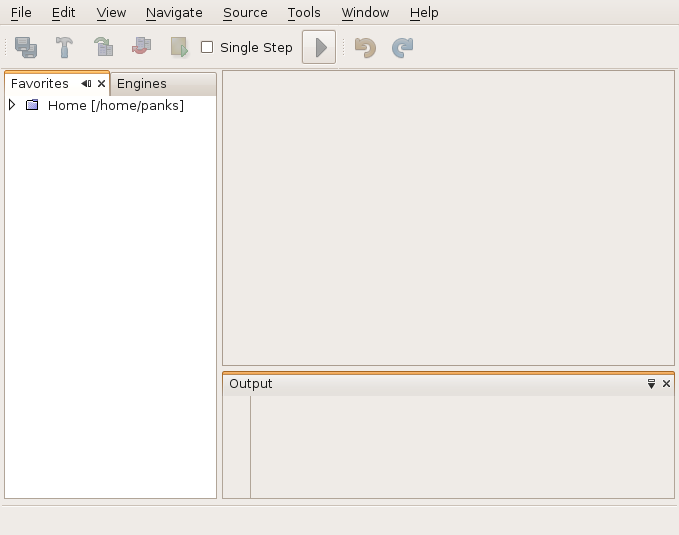
\includegraphics[scale=0.60]
{blide/dia/Blide1}
\caption[] {}
  \label{fig:blide1}
\end{center}
\end{figure}
 
